\documentclass[aspectratio=169,11pt]{beamer}

\usetheme{Madrid}
\usecolortheme{default}
\usepackage{amsmath,amssymb}
\usepackage{booktabs}
\usepackage{tikz}
\usetikzlibrary{arrows.meta,positioning}

\title{Fundamentals of Set Theory}
\subtitle{Sets, Set Builder Form, Types, Operations, Counting, and Hasse Diagrams}
\author{}
\date{}

\begin{document}

\begin{frame}
  \titlepage
\end{frame}

\section{Sets}

\begin{frame}{What Is a Set?}
A \alert{Set} is a well-defined collection of distinct objects, called
\alert{Elements} or \alert{Members}.

\[
 A=\{1,2,3,4\}
\]

\begin{itemize}
  \item \(2\in A\) means that 2 is an element of \(A\).
  \item \(7\notin A\) means that 7 is not an element of \(A\).
  \item Order does not matter: \(\{1,2,3\}=\{3,2,1\}\).
  \item Repeated elements are counted only once:
        \(\{1,1,2\}=\{1,2\}\).
\end{itemize}
\end{frame}

\begin{frame}{Ways to Represent a Set}
\textbf{1. Roster (listing) form}
\[
  V=\{a,e,i,o,u\}
\]

\textbf{2. Descriptive form}

\(V\) is the Set of vowels in the English alphabet.

\textbf{3. Set-builder form}
\[
  V=\{x\mid x\text{ is a vowel in the English alphabet}\}
\]
The symbol \(\mid\) means ``such that.''
\end{frame}

\section{Set Builder Form}

\begin{frame}{Set-Builder Form}
Set-builder notation describes a Set by stating the property its elements
must satisfy.

\[
  A=\{x\in\mathbb{Z}\mid -2\leq x\leq 2\}
\]

This means: \(A\) contains all integers from \(-2\) to \(2\).

\[
  A=\{-2,-1,0,1,2\}
\]

\textbf{General pattern}
\[
  \{x\in U\mid P(x)\}
\]
where \(U\) is the universe of possible values and \(P(x)\) is the condition
that an element must satisfy.
\end{frame}

\begin{frame}{More Set-Builder Examples}
\begin{itemize}
  \item Even natural numbers:
  \[
    E=\{x\in\mathbb{N}\mid x=2k\text{ for some }k\in\mathbb{N}\}.
  \]
  \item Positive integers less than 6:
  \[
    B=\{x\in\mathbb{Z}\mid 0<x<6\}=\{1,2,3,4,5\}.
  \]
  \item Squares of the first five natural numbers (starting at 1):
  \[
    S=\{n^2\mid n\in\mathbb{N},\,1\leq n\leq5\}
      =\{1,4,9,16,25\}.
  \]
\end{itemize}
\end{frame}

\section{Types of Sets}

\begin{frame}{Common Types of Sets}
\begin{description}
  \item[Empty set] A set with no elements: \(\varnothing\) or \(\{\}\).
  \item[Singleton set] A set with exactly one element: \(\{0\}\).
  \item[Finite set] A set with a limited number of elements: \(\{a,b,c\}\).
  \item[Infinite set] A set with infinitely many elements:
        \(\mathbb{N}=\{1,2,3,\ldots\}\).
  \item[Equal sets] Sets containing exactly the same elements.
  \item[Equivalent sets] Sets having the same number of elements.
\end{description}
\end{frame}

\begin{frame}{More Types: Subsets and Disjoint Sets}
\begin{itemize}
  \item \(A\) is a \alert{subset} of \(B\), written \(A\subseteq B\), if
        every element of \(A\) is also in \(B\).
  \[
    \{1,2\}\subseteq\{1,2,3\}.
  \]
  \item A \alert{proper subset}, \(A\subsetneq B\), is a subset that is not
        equal to \(B\).
  \item Two sets are \alert{disjoint} if they have no common elements:
  \[
    A\cap B=\varnothing.
  \]
  \item The \alert{power set} \(\mathcal{P}(A)\) is the set of all subsets
        of \(A\). If \(A=\{a,b\}\), then
  \[
    \mathcal{P}(A)=\{\varnothing,\{a\},\{b\},\{a,b\}\}.
  \]
\end{itemize}
\end{frame}

\section{Set Operations}

\begin{frame}{Basic Set Operations}
Let \(A=\{1,2,3\}\) and \(B=\{3,4,5\}\).

\begin{description}
  \item[Union] Elements in \(A\), in \(B\), or in both:
  \[
    A\cup B=\{1,2,3,4,5\}.
  \]
  \item[Intersection] Elements common to both:
  \[
    A\cap B=\{3\}.
  \]
  \item[Difference] Elements in the first set but not the second:
  \[
    A\setminus B=\{1,2\},\qquad B\setminus A=\{4,5\}.
  \]
\end{description}
\end{frame}

\begin{frame}{Complement and Key Laws}
If the universal set is \(U\), the complement of \(A\) is
\[
  A^c=U\setminus A.
\]

Important identities:
\begin{align*}
 A\cup\varnothing&=A & A\cap U&=A\\
 A\cup A&=A & A\cap A&=A\\
 A\cup A^c&=U & A\cap A^c&=\varnothing
\end{align*}

\textbf{De Morgan's laws}
\[
 (A\cup B)^c=A^c\cap B^c,\qquad
 (A\cap B)^c=A^c\cup B^c.
\]
\end{frame}

\section{Inclusion--Exclusion Principle}

\begin{frame}{Inclusion--Exclusion Principle}
The inclusion--exclusion principle prevents elements in an overlap from
being counted more than once.

For two finite sets:
\[
  \boxed{|A\cup B|=|A|+|B|-|A\cap B|}
\]

\textbf{Example}

In a class, 18 students study Mathematics, 12 study Physics, and 5 study
both. The number studying at least one subject is
\[
  |M\cup P|=18+12-5=\boxed{25}.
\]
\end{frame}

\begin{frame}{Inclusion--Exclusion for Three Sets}
For three finite sets:
\begin{align*}
|A\cup B\cup C|={}&|A|+|B|+|C|\\
&-|A\cap B|-|A\cap C|-|B\cap C|\\
&+|A\cap B\cap C|.
\end{align*}

\textbf{Why add the triple intersection back?}

The elements in all three sets are:
\begin{itemize}
  \item counted three times in the first line;
  \item subtracted three times in the second line;
  \item therefore counted zero times so far.
\end{itemize}
Adding the triple intersection once gives each such element a final count of 1.
\end{frame}

\section{Hasse Diagrams}

\begin{frame}{Partially Ordered Sets}
A \alert{partial order} is a relation \(\preceq\) that is:
\begin{itemize}
  \item reflexive: \(a\preceq a\);
  \item antisymmetric: if \(a\preceq b\) and \(b\preceq a\), then \(a=b\);
  \item transitive: if \(a\preceq b\) and \(b\preceq c\), then \(a\preceq c\).
\end{itemize}

A set together with a partial order is called a \alert{partially ordered set}
(or \alert{poset}).

Example: the positive divisors of 6, ordered by divisibility:
\[
  D=\{1,2,3,6\},\qquad a\preceq b\iff a\mid b.
\]
\end{frame}

\begin{frame}{What Is a Hasse Diagram?}
A Hasse diagram is a simplified drawing of a finite partially ordered set.

\begin{itemize}
  \item Smaller elements are placed lower and larger elements higher.
  \item A line joins \(a\) to \(b\) when \(b\) covers \(a\).
  \item Reflexive loops and edges implied by transitivity are omitted.
  \item The diagram represents the order relation, not necessarily numerical
        size.
\end{itemize}
\end{frame}

\begin{frame}{Example Hasse Diagram: Divisors of 6}
The order is divisibility. Thus \(1\mid2\), \(1\mid3\), \(2\mid6\), and
\(3\mid6\).

\begin{center}
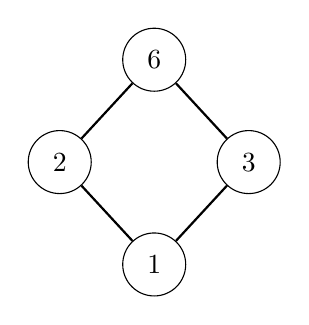
\begin{tikzpicture}[
  every node/.style={circle,draw,minimum size=8mm},
  edge/.style={thick}
]
\node (one) at (0,0) {1};
\node (two) at (-1.2,1.3) {2};
\node (three) at (1.2,1.3) {3};
\node (six) at (0,2.6) {6};
\draw[edge] (one)--(two);
\draw[edge] (one)--(three);
\draw[edge] (two)--(six);
\draw[edge] (three)--(six);
\end{tikzpicture}
\end{center}

Neither 2 nor 3 is above the other: they are incomparable under divisibility.
\end{frame}

\begin{frame}{How to Construct a Hasse Diagram}
\begin{enumerate}
  \item List the elements of the poset.
  \item Determine which pairs are related by the partial order.
  \item Remove reflexive relations.
  \item Remove relations that follow from transitivity.
  \item Place lower elements below higher elements and draw the remaining
        cover relations.
\end{enumerate}

\textbf{Tip:} For divisibility, connect \(a\) to \(b\) when \(a\mid b\)
and there is no listed element strictly between them in the divisibility
order.
\end{frame}

\begin{frame}{Quick Review}
\begin{itemize}
  \item A set is a well-defined collection of distinct elements.
  \item Set-builder notation describes elements through a condition.
  \item Common set types include empty, finite, infinite, subset, and power set.
  \item Union, intersection, difference, and complement are basic operations.
  \item Inclusion--exclusion counts unions without double-counting overlaps.
  \item Hasse diagrams display cover relations in a partially ordered set.
\end{itemize}
\end{frame}

\begin{frame}{Practice Questions}
\begin{enumerate}
  \item Write \(\{2,4,6,8,10\}\) in set-builder form.
  \item If \(A=\{1,2,3,4\}\) and \(B=\{3,4,5\}\), find
        \(A\cup B\), \(A\cap B\), and \(A\setminus B\).
  \item In a group, 20 people like tea, 15 like coffee, and 7 like both.
        How many like tea or coffee?
  \item Draw the Hasse diagram for \(\{1,2,4,8\}\) ordered by divisibility.
\end{enumerate}
\end{frame}

\end{document}
